% \pagebreak[4]
% \hspace*{1cm}
% \pagebreak[4]
% \hspace*{1cm}
% \pagebreak[4]

\chapter{Giới thiệu tổng quan}
\ifpdf
    \graphicspath{{Chapter1/Chapter1Figs/PNG/}{Chapter1/Chapter1Figs/PDF/}{Chapter1/Chapter1Figs/}}
\else
    \graphicspath{{Chapter1/Chapter1Figs/EPS/}{Chapter1/Chapter1Figs/}}
\fi
\markboth{\MakeUppercase{\thechapter. Giới thiệu tổng quan}}{Chương \thechapter. Giới thiệu tổng quan}
\section{Mục tiêu và động lực chọn đề tài}
Trong những năm gần đây, cùng với sự phát triển của công nghệ thông tin, các lĩnh vực liên quan đến kỹ thuật số cũng đang có tốc độ phát triển chóng mặt. Các thiết bị kỹ thuật số như máy ảnh, máy quay phim kỹ thuật số, camera số, điện thoại di động có chức năng chụp hình, ... đang ngày càng phổ biến và không ngừng gia tăng về số lượng. Chính điều này đã làm sản sinh ra một lượng thông tin số khổng lồ bao gồm hình ảnh, video, v.v... Do đó, nhu cầu truy vấn thông tin từ kho dữ liệu hình ảnh, video ngày càng bức thiết hơn bao giờ hết.\\
Mục tiêu của luận văn này nhằm xây dựng một hệ thống truy vấn ảnh trên tập dữ liệu lớn, trong đó quá trình truy vấn hoàn toàn dựa trên nội dung của ảnh và kết quả phải được trả về gần như ngay lập tức với cơ sở dữ liệu gồm hàng triệu hình ảnh chưa được gán nhãn. Hệ thống này tập trung vào giải quyết vấn đề về tìm kiếm một đối tượng cụ thể như một địa điểm, một bức tranh, một bìa sách, v.v... Những đối tượng này có thể được chụp trong các điều kiện khác nhau như góc chụp, ánh sáng, kích thước hay bị che khuất. Do đó mục đích của hệ thống không phải là trả về những hình ảnh chụp gần giống nhau như chụp trong cùng một khung cảnh mà là trả về những hình ảnh có chứa đối tượng cần tìm. Ví dụ như khi đưa vào một bức hình có chứa Nhà thờ Đức Bà, kết quả trả về sẽ những bức hình có chứa nhà thờ Đức Bà chứ không phải trả về những nhà thờ có kiến trúc gần giống với Nhà thờ Đức Bà.\\
Những hệ thống truy vấn ảnh trên tập dữ liệu lớn có rất nhiều ứng dụng trong thực tế. Chúng tôi sẽ liệt kê sơ lược một vài ứng dụng trong phần tiếp theo.\\

\section{Một vài hướng ứng dụng thực tế của hệ thống}

Trong cuộc sống, ta có thể dễ dàng bắt gặp những ứng dụng vô cùng hữu ích của các hệ thống truy vấn đối tượng trên ảnh. Dưới đây là một vài hướng ứng dụng cụ thể:\\
\textbf{Nhận dạng đối tượng, sản phẩm.} Với sự phổ biến của điện thoại thông minh và internet, một người có thể dễ dàng dùng điện thoại chụp một tấm hình và hỏi hệ thống về thông tin của đối tượng trong tấm hình đó. Ví dụ, tại một cửa hàng, một người mua hàng có thể tham khảo giá của một sản phẩm tại các cửa hàng khác; trong thư viện, một độc giả có thể tìm được những cuốn sách nào chứa hình ảnh mình quan tâm; khi đi thăm bảo tàng, du khách có thể tìm kiếm thêm thông tin về một hiện vật trong đó, v.v...\\
\textbf{Nhận dạng địa điểm.} Vị trí địa lý của nơi chụp tấm hình cũng có thể được xác định bằng việc truy vấn thông tin của đối tượng trong hình từ những cơ sở dữ liệu lớn chứa hình ảnh và thông tin vị trí như Google Street View hay kho hình ảnh có lưu kèm thông tin GPS. Hệ thống này có thể là một giải pháp thay thế rẻ tiền cho các thiết bị có GPS. Chẳng hạn, khi một du khách đến một nơi mà anh ta chưa bao giờ đặt chân tới nhưng lại không GPS hay bản đồ, anh ta có thể chụp một tấm hình của một tòa nhà hay những cảnh tại nơi đó để xác định được vị trí chính xác của mình.\\
\textbf{Tìm kiếm và quản lý kho dữ liệu video.} Hàng ngày, một lượng lớn dữ liệu video được sinh ra và ta không thể nào quản lý hết được nội dung của chúng. Ví dụ, một hãng phim hay truyền hình muốn tìm kiếm tất cả các đoạn quảng cáo có liên quan đến một nhãn hiệu sản phẩm mà họ đã từng phát trong vài năm gần đây, một hệ thống truy vấn ảnh sẽ dễ dàng thực hiện điều này chỉ với một bức hình của sản phẩm.\\
\textbf{Gán nhãn ảnh tự động.} Những tấm ảnh có thể được gán nhãn một cách tự động về địa điểm hay đối tượng trong hình để dễ dàng cho việc tìm kiếm và quản lý sau này. Ví dụ, người dùng có thể dễ dàng tìm kiếm được những bức hình chụp tại một địa điểm nào đó mà không cần biết nó nằm trong album nào hay được chụp ngày nào. Những hệ thống lớn lưu trữ ảnh lớn như của Facebook có thể dễ dàng phát hiện và gán nhãn khuôn mặt người nhưng vẫn chưa thể nhận dạng được địa điểm mà tấm hình được chụp từ nội dung chứa trong hình.\\
\textbf{Sử dụng trong quảng cáo theo ngữ cảnh.} Rất nhiều công ty quảng cáo đặt màn hình tại nơi công cộng để quảng cáo cho các sản phẩm của mình nhưng các quảng cáo này chưa thực sự hướng người dùng và kém hiệu quả. Việc sử dụng một hệ thống có thể quảng cáo theo ngữ cảnh và hướng đúng đối tượng người dùng sẽ giúp việc quảng cáo hiệu quả hơn. Ví dụ, một camera trong thang máy có thể tự động phát hiện được những sản phẩm người đi thang máy đang dùng như nhãn hiệu chai nước họ đang uống, nhãn hiệu quần áo họ đang mặc,... để lựa chọn được những quảng cáo phù hợp với đối tượng người dùng và phát trên màn hình.\\
\textbf{Tăng tính tương tác thực tế.} Với sự ra đời của các sản phẩm công nghệ gần gũi với cuộc sống như Google Glass, việc nhận dạng đối tượng trong thời gian thực sẽ mang đến nhiều thông tin hữu ích cho người dùng.\\
\textbf{Hỗ trợ cho các hệ thống thị giác máy tính khác.} Hệ thống truy vấn đối tượng có thể được dùng để hỗ trợ cho các hệ thống thị giác máy tính khác. Một ví dụ điển hình là hệ thống tự động tái tạo hình ảnh ba chiều sẽ cần gom cụm các hình ảnh của cùng một đối tượng từ một tập dữ liệu lớn.\\


%Thử nghiệm trích dẫn \cite{Ahamed2010FTMforPervasiveEnvironments}. Trích dẫn tên tác giả \citet{Ahamed2010FTMforPervasiveEnvironments}. Trích dẫn đầy đủ 
%\citet*{Ahamed2010FTMforPervasiveEnvironments}. 
%
%Để học thêm về cách sử dụng gói trích dẫn natbib, các bạn cần đọc thêm tại đây: http://casa.colorado.edu/\~danforth/comp/tex/tutorial.html
%
%Here is an equation\footnote{the notation is explained in the nomenclature section :-)}:
%\begin{eqnarray}
%CIF: \hspace*{5mm}F_0^j(a) &=& \frac{1}{2\pi \iota} \oint_{\gamma} \frac{F_0^j(z)}{z - a} dz
%\end{eqnarray}
%\nomenclature[zcif]{$CIF$}{Cauchy's Integral Formula}                                % first letter Z is for Acronyms 
%\nomenclature[aF]{$F$}{complex function}                                                   % first letter A is for Roman symbols
%\nomenclature[gp]{$\pi$}{ $\simeq 3.14\ldots$}                                             % first letter G is for Greek Symbols
%\nomenclature[gi]{$\iota$}{unit imaginary number $\sqrt{-1}$}                      % first letter G is for Greek Symbols
%\nomenclature[gg]{$\gamma$}{a simply closed curve on a complex plane}  % first letter G is for Greek Symbols
%\nomenclature[xi]{$\oint_\gamma$}{integration around a curve $\gamma$} % first letter X is for Other Symbols
%\nomenclature[rj]{$j$}{superscript index}                                                       % first letter R is for superscripts
%\nomenclature[s0]{$0$}{subscript index}                                                        % first letter S is for subscripts

\section{Những thách thức đặt ra}
 Để giải quyết bài toán truy vấn đối tượng trên tập dữ liệu ảnh lớn, có rất nhiều thách thức được đặt ra. Dưới đây chúng tôi sẽ trình bày một vài thách thức trong bài toán này:\\
 \begin{figure}[!htbp]
  \begin{center}
    \leavevmode
    \ifpdf
      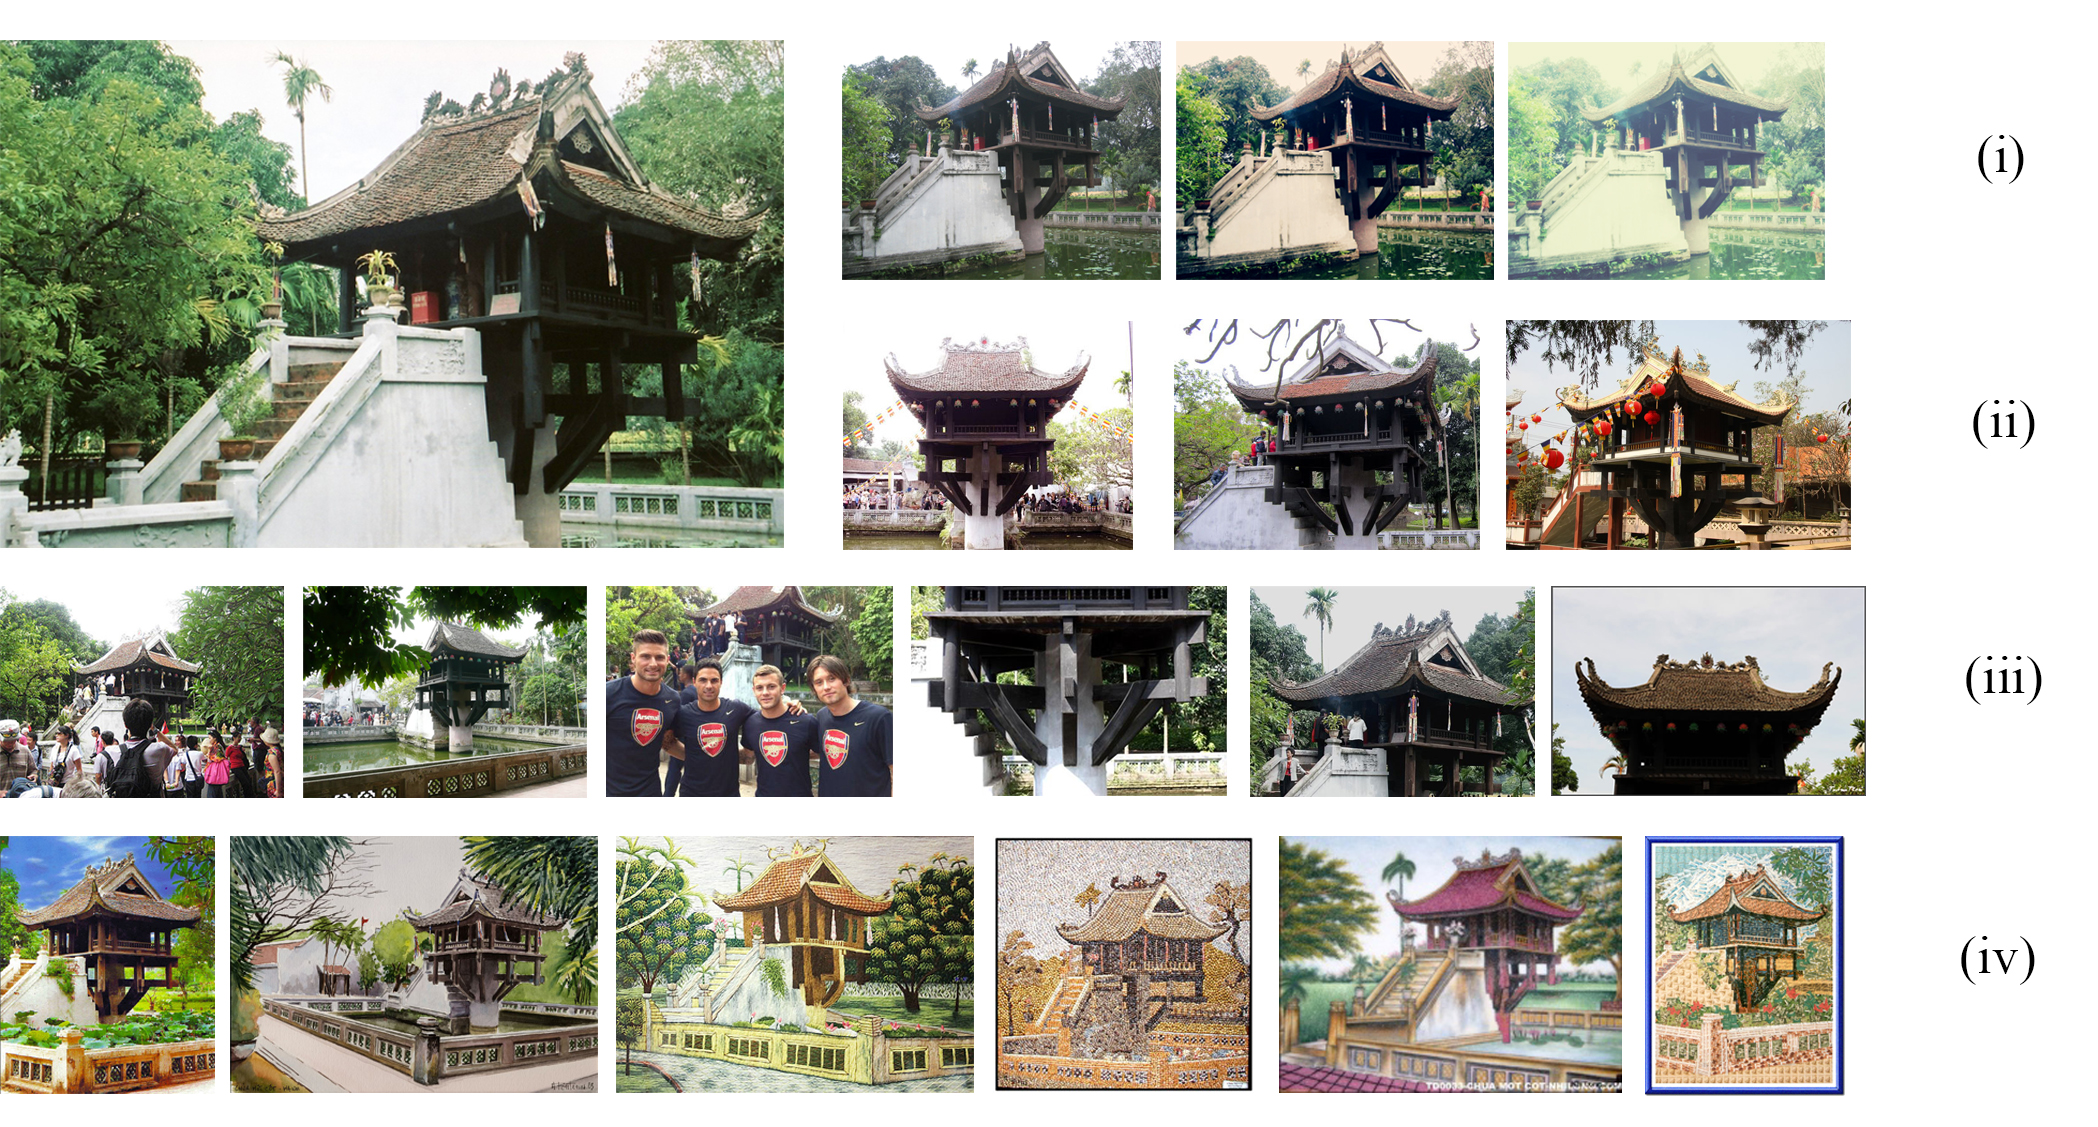
\includegraphics[scale=0.20]{chuaMotCot}
    \else
      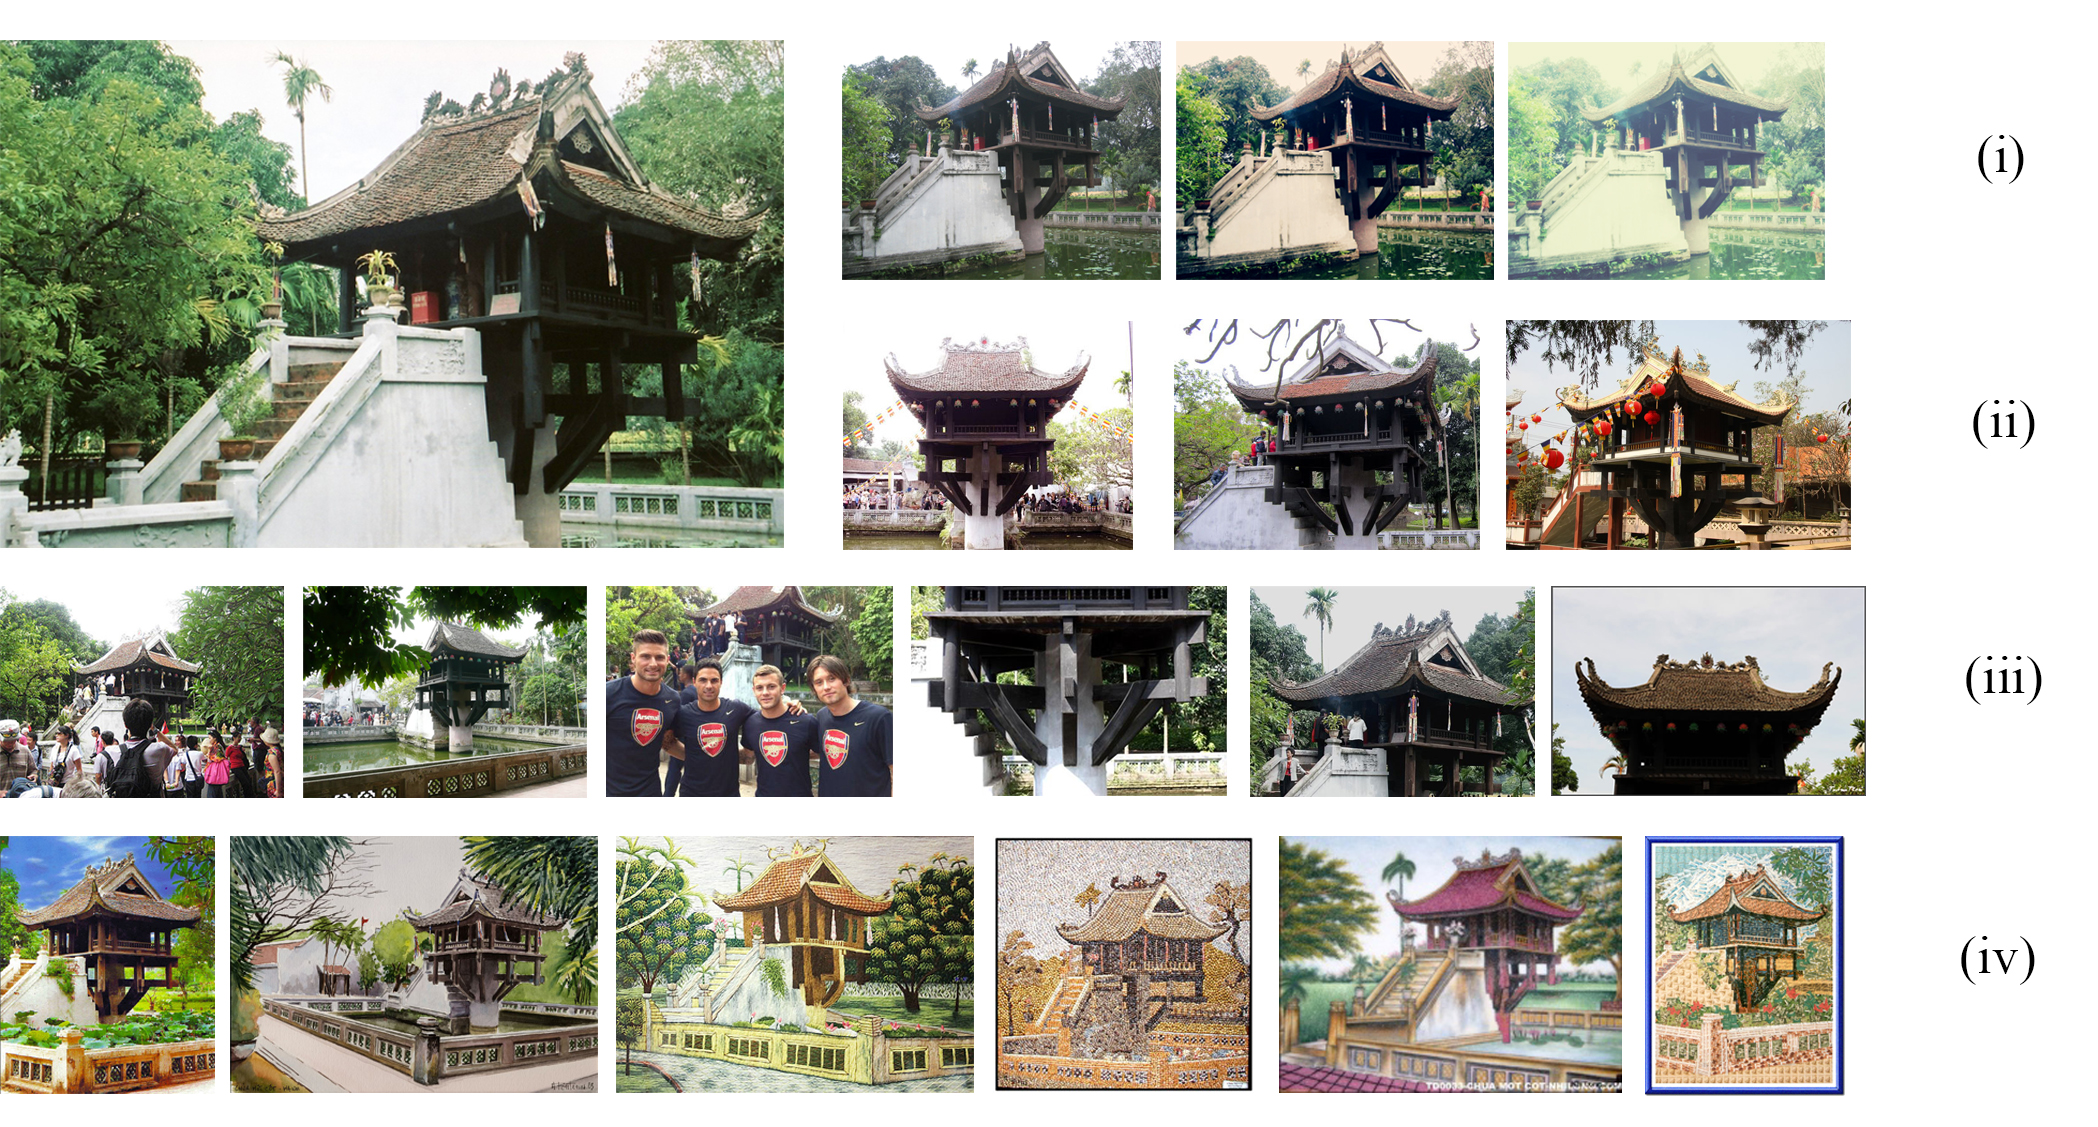
\includegraphics[scale=0.20]{chuaMotCot}
    \fi
    \caption[Những thay đổi bề ngoài của đối tượng trên ảnh]{\textbf{Những thay đổi bề ngoài của đối tượng trên ảnh.} \textit{(i) Hình ảnh đối tượng trong các điều kiện chiếu sáng khác nhau. (ii) Hình ảnh đối tượng dưới các góc chụp khác nhau. (iii) Đối tượng bị che khuất hay hình ảnh đối tượng bị cắt ghép. (iv) Hình ảnh đối tượng trong các ấn phẩm, bản in, bản vẽ.}}
    \label{FigTemple}
  \end{center}
\end{figure} 
 \textbf{Sự biến đổi bề ngoài của đối tượng trong hình ảnh.} Một hệ thống truy vấn đối tượng trên hình ảnh cần phải trả về được các hình ảnh có chứa đối tượng quan tâm bất chấp mọi thay đổi trên bên ngoài của đối tượng. Những thay đổi đó có thể đến từ rất nhiều nguyên nhân khác nhau. Đó có thể do tác động từ các yếu tố bên ngoài khi chụp hình như điều kiện chiếu sáng, góc chụp của camera hay những tùy chỉnh khác nhau của các camera về độ tương phản, độ phân giải, màu sắc,... Cùng với đó là những hình ảnh của đối tượng được chụp với góc xoay, kích thước hình hay tỉ lệ khác nhau. Hoặc có những trường hợp đối tượng bị che khuất, cắt ghép, v.v... hoặc đối tượng được thể hiện trên các ấn phẩm, bản in, bản vẽ nên bị thay đổi về màu sắc và chi tiết. Một vài dạng thay đổi kể trên được thể hiện qua Hình \ref{FigTemple}. Còn một trường hợp nữa là do những thay đổi từ chính bản thân đối tượng do các điều kiện bên ngoài ví dụ như đối tượng bị cũ đi hay bị xuống cấp theo thời gian.\\ 
 \textbf{Các loại đặc tính vật lý khác nhau trên mỗi đối tượng.} Dựa trên các đặc tính vật lý người ta chia đối tượng thành các loại khác nhau. Có những đối tượng mà đặc tính thể hiện rõ nét nhất qua cấu trúc bề mặt, nhưng có cái lại qua màu sắc hay hình dạng, v.v... Ví dụ như với những con bướm, đặc trưng cho chúng không phải là hình dạng, kích cỡ vì đa phần các loài bướm đều có hình dạng, kích cỡ gần giống nhau mà ở đây là các họa tiết, màu sắc trên cánh bướm; Hay với những loại lá cây thì đặc trưng về màu sắc, họa tiết lại không cung cấp nhiều thông tin bằng hình dạng của lá.\\
 \textbf{Kích cỡ của tập dữ liệu lớn.} Tập dữ liệu hình ảnh lớn thường bao gồm hàng triệu bức ảnh, vậy nên để người dùng có thể tương tác trực tiếp với hệ thống thông qua một thiết bị phía client như điện thoại di động thì đòi hỏi truy vấn phải được trả về trong thời gian ngắn chấp nhận được. Do đó cần phải có một thuật toán nhận dạng hiệu quả, chi phí thấp. Đồng thời những hình ảnh cũng phải được xử lý để lưu trữ sao cho tiết kiệm nhất để phù hợp với kích cỡ của RAM vì nếu lưu trữ trên ổ cứng sẽ mất rất nhiều thời gian để truy xuất và không thể đạt được yêu cầu về thời gian.\\

\section{Cấu trúc luận văn}
Trong phần này, chúng tôi sẽ trình bày cấu trúc phần còn lại của luận văn và những vấn đề được thảo luận ở phần kế tiếp. Các nội dung sẽ được trình bày ở phần kế tiếp bao gồm:


